% formato FRONTE RETRO
\documentclass[epsfig,a4paper,11pt,titlepage,twoside,openany]{book}
\usepackage{style/thesis_style}

%% BEGIN DOCUMENT

\begin{document}
\def\biblio{}

  % nessuna numerazione
  \pagenumbering{gobble} 
  \pagestyle{plain}

\graphicspath{first_page/}

\thispagestyle{empty}

\begin{center}
  \begin{figure}[h!]
    \centerline{
\psfig{file=first_page/marchio_unitrento_colore_it_202002.png,width=0.6\textwidth}}
  \end{figure}

  \vspace{2 cm} 

  \LARGE{Department of Information Engineering and Computer Science\\}

  \vspace{1 cm} 
  \Large{Bachelor's Degree in Computer Science
  }

  \vspace{2 cm} 
  \Large\textsc{Final dissertation\\} 
  \vspace{1 cm} 
  \Huge\textsc{The emotional impact of the Covid-19\\}
  \vspace{.3 cm}
  \Large{\it{Studying the emotional impact of the Covid-19 pandemic using social media}}


  \vspace{2 cm} 
  \begin{tabular*}{\textwidth}{ c @{\extracolsep{\fill}} c @{\extracolsep{\fill}} c }
  \vspace{.3 cm} 
  \Large{Supervisor} & \Large{Co-Supervisor} & \Large{Student}\\
  \vspace{.3 cm} 
  \Large{Alberto Montresor} & \Large{Cristian Consonni} & \Large{Simone Alghisi}\\
  \vspace{.3 cm} 
   & \Large{David Laniado} & \\
  \end{tabular*}

  \vspace{2 cm} 

  \Large{Academic year 2020/2021}
  
\end{center}



  \clearpage

\newgeometry{paperheight=29.7cm,paperwidth=21cm,outer=1.5cm,inner=2.5cm,top=2cm,bottom=2cm}
%%%%%%%%%%%%%%%%%%%%%%%%%%%%%%%%%%%%%%%%%%%%%%%%%%%%%%%%%%%%%%%%%%%%%%%%%%
%%%%%%%%%%%%%%%%%%%%%%%%%%%%%%%%%%%%%%%%%%%%%%%%%%%%%%%%%%%%%%%%%%%%%%%%%%
%% Nota
%%%%%%%%%%%%%%%%%%%%%%%%%%%%%%%%%%%%%%%%%%%%%%%%%%%%%%%%%%%%%%%%%%%%%%%%%%
%% Sezione Ringraziamenti opzionale
%%%%%%%%%%%%%%%%%%%%%%%%%%%%%%%%%%%%%%%%%%%%%%%%%%%%%%%%%%%%%%%%%%%%%%%%%%
%%%%%%%%%%%%%%%%%%%%%%%%%%%%%%%%%%%%%%%%%%%%%%%%%%%%%%%%%%%%%%%%%%%%%%%%%%
  %\thispagestyle{empty}

\begin{center}
  {\bf \Huge Special thanks}
\end{center}

\vspace{4cm}


\emph{
  ...thanks to...
}

  \clearpage
  \pagestyle{plain} % nessuna intestazione e pie pagina con numero al centro


  % inizio numerazione pagine in numeri arabi
  \mainmatter

%%%%%%%%%%%%%%%%%%%%%%%%%%%%%%%%%%%%%%%%%%%%%%%%%%%%%%%%%%%%%%%%%%%%%%%%%%
%%%%%%%%%%%%%%%%%%%%%%%%%%%%%%%%%%%%%%%%%%%%%%%%%%%%%%%%%%%%%%%%%%%%%%%%%%
%% Nota
%%%%%%%%%%%%%%%%%%%%%%%%%%%%%%%%%%%%%%%%%%%%%%%%%%%%%%%%%%%%%%%%%%%%%%%%%%
%% Si ricorda che il numero massimo di facciate e' 30.
%% Nel conteggio delle facciate sono incluse 
%%   indice
%%   sommario
%%   capitoli
%% Dal conteggio delle facciate sono escluse
%%   frontespizio
%%   ringraziamenti
%%   allegati
%%	 bibliografia
%%%%%%%%%%%%%%%%%%%%%%%%%%%%%%%%%%%%%%%%%%%%%%%%%%%%%%%%%%%%%%%%%%%%%%%%%%
%%%%%%%%%%%%%%%%%%%%%%%%%%%%%%%%%%%%%%%%%%%%%%%%%%%%%%%%%%%%%%%%%%%%%%%%%%

    % indice
    \tableofcontents
    \clearpage



    % gruppo per definizone di successione capitoli senza interruzione di pagina
    \begingroup
      % nessuna interruzione di pagina tra capitoli
      % ridefinizione dei comandi di clear page
      \renewcommand{\cleardoublepage}{} 
      \renewcommand{\clearpage}{} 
      % redefinizione del formato del titolo del capitolo
      % da formato
      %   Capitolo X
      %   Titolo capitolo
      % a formato
      %   X   Titolo capitolo
      
      \titleformat{\chapter}
        {\normalfont\Huge\bfseries}{\thechapter}{1em}{}
        
      \titlespacing*{\chapter}{0pt}{0.59in}{0.02in}
      \titlespacing*{\section}{0pt}{0.20in}{0.02in}
      \titlespacing*{\subsection}{0pt}{0.10in}{0.02in}
      
      % sommario
      %%%%%%%%%%%%%%%%%%%%%%%%%%%%%%%%%%%%%%%%%%%%%%%%%%%%%%%%%%%%%%%%%%%%%%%%%%
%%%%%%%%%%%%%%%%%%%%%%%%%%%%%%%%%%%%%%%%%%%%%%%%%%%%%%%%%%%%%%%%%%%%%%%%%%
%% Nota
%%%%%%%%%%%%%%%%%%%%%%%%%%%%%%%%%%%%%%%%%%%%%%%%%%%%%%%%%%%%%%%%%%%%%%%%%%
%% Sommario e' un breve riassunto del lavoro svolto dove si descrive 
%% l’obiettivo, l’oggetto della tesi, le metodologie e 
%% le tecniche usate, i dati elaborati e la spiegazione delle conclusioni 
%% alle quali siete arrivati.
%% Il sommario dell’elaborato consiste al massimo di 3 pagine e deve contenere le seguenti informazioni: 
%%   contesto e motivazioni
%%   breve riassunto del problema affrontato
%%   tecniche utilizzate e/o sviluppate
%%   risultati raggiunti, sottolineando il contributo personale del laureando/a
%%%%%%%%%%%%%%%%%%%%%%%%%%%%%%%%%%%%%%%%%%%%%%%%%%%%%%%%%%%%%%%%%%%%%%%%%%
%%%%%%%%%%%%%%%%%%%%%%%%%%%%%%%%%%%%%%%%%%%%%%%%%%%%%%%%%%%%%%%%%%%%%%%%%%

\chapter*{Abstract} % senza numerazione
\label{abstract}  

\addcontentsline{toc}{chapter}{Abstract} % da aggiungere comunque all'indice

This dissertation describes in detail the activity performed during my two-month traineeship at the Big Data Department of Eurecat - Centro Tecnológico de Catalunya, which was supervised by Cristian Consonni and David Laniado.

The purpose of the project was to analyze the emotions emerging from Twitter messages during the pandemic, in order to understand how people felt over the whole period. Based on the result obtained from this research, it may be possible to determine which countermeasures better handled the situation while offering the best possible trade-off between people's satisfaction and the reduction of the spread of the disease.

For this project I have
    
    \begin{itemize}
    	\item retrieved over 6TB of data from Twitter
    	\item analyzed users' emotions using state-of-the-art libraries (EmoLex, LIWC)
    	\item studied which emotions were expressed by a large group of users in 4 languages (ca, en, es, it)
    	\item studied how the emotions expressed by users can vary based on their demographic characteristic, including inferred age and gender
    	\item studied how the emotions expressed by users can vary based on their geographical provenance (at national and regional level)
    \end{itemize}

The dataset used for the project is the echen102/COVID-19-TweetIDs, an ongoing collection of over 1 billion tweet IDs available on GitHub. The selected tweets are either related to specific accounts, or sampled real-time from the Twitter API because they matched a defined set of keywords.

In order to start the analysis, I was asked to retrieve the tweets from January 2020 to March 2021 using Twarc. In fact, to comply with Twitter's term of service, the dataset contains only the ID of the original tweet; however, is possible to get the associated information using the Twitter's API and a Twitter Developer Account.

After collecting the data, we decided to group the tweets first based on their language, to perform a targeted analysis on a restricted set (Catalan, English, Italian and Spanish); secondly per week, for better data visualization and to average the results.

In order to understand which emotions were expressed in a single tweet, we decided to use the NRC Word-Emotion Association Lexicon (aka EmoLex). Emolex is a list of English words and their associations with eight basic emotions (anger, fear, anticipation, trust, surprise, sadness, joy, and disgust) and two sentiments (negative and positive). Furthermore, we decided to validate the results obtained from EmoLex with LIWC, a widely used computerized text analysis program that outputs the percentage of words in a given text that falls into one or more categories.

To reduce the possible bias of particularly active users, we decided to follow one of the approaches discussed by Aiello et al., in particular we have considered
	
\begin{itemize}
	\item emotions in a binary way (e.g. whether in a given week the user expressed joy or not)
	\item users over tweets (e.g. the number of unique users, instead of tweets, that expressed joy in a week)
\end{itemize}

For the first sentiment analysis, tweets belonging to a given language were analyzed over the whole period. In particular, we decided to normalize the obtained results using the z-score and to manually retrieve some peaks to study the most used words for that particular language.

To understand how differently men and women perceived the pandemic, we decided to use\\ m3inference, a deep learning system for demographic inference (gender, age, and person/organization) implemented on PyTorch. Only those users that the system inferred with a confidence grater or equal to 0.95 were considered valid and used for the next sentiment analysis.

Given the fact that m3inference also outputs a prediction for the users' age, we decided to analyze the emotions of people belonging to different age brackets. In particular, we considered only users with less than forty years and with at least forty years. As before, we took into account only those users that the system predicted with a confidence of at least 0.95. 

Finally, we used Twitter location field to analyze users from the same geographical area. To overcome the absence of constraints to specify a location, we retrieved the position of the users using address geocoding, the process of taking a text-based description of a location and returning its geographic coordinates. In particular, we used Nominatim to access the data made available by OpenStreetMap(OSM).

The analysis of the data revealed some first interesting results:

\begin{itemize}
	\item first of all, there are cases when the course of the emotions seems to be the same. In particular, when one emotion increases, so do the others. This could happen because on some days users are simply more emotional and tend to use more words. Because of that, the probability of conveying more emotions increases. Furthermore, more emotions could be associated to a single word, so this also explains why some emotions are always more frequently expressed than the others.
	\item secondly, if we consider the English tweets it seems that women tend to express joy more frequently in their tweets. The same goes for sadness and fear, but in this case the difference is less marked. Finally, anger seems to be slightly more expressed by men, but the lines tend to overlap for the majority of the considered period of time.
	\item then, always from the analysis of the English tweets, we noticed that users with less than forty years tend to express fewer emotions w.r.t. users with at least forty years. This could be due to the fact that younger users prefer to write shorter tweets, use a lot of emoticons or slang, or they are simply more inexpressive.
	\item finally, we were able to understand the proportion of Italian users for each state. However, even if it is indeed possible to map manually certain emotional peaks to particular events that occurred around the same time, we still lack a way to perform this method in a more valid and reliable way.
\end{itemize}

During the course of the project I had the possibility to personally contribute to the improvement of m3inference on GitHub, by opening a pull request to solve some issues while downloading images from Twitter.

In the end, I was only able to scratch the surface of this research field, because the amount of data to analyze was really impressive. In any case, I hope that my contribution could be a good starting point for further studies and I would really like to continue researching about this topic in the future.

      %%%%%%%%%%%%%%%%%%%%%%%%%%%%%%%%
      % lista dei capitoli
      %
      % \input oppure \include
      %
      \chapter{Introduction}
\label{cha:intro}

The COVID-19 pandemic is having a huge impact on our lives, that goes beyond the direct effects of the virus. Besides the fear of infection, lockdown measures adopted by many countries are limiting the possibility to move, work, have contact with others, and are creating a situation of economic crisis and generalized uncertainty about the future. The psychological effects of this unprecedented situation need to be studied.

\paragraph{Context and motivations}

During this year, everyone's daily life changed significantly and we had to adapt to restrictive measures in order to stop the disease, whether we liked it or not. The research proposed by Eurecat (Centro Tecnológico de Catalunya) really caught my eye: the possibility to study how people perceived all of this situation and to better understand which measures were more welcomed than others was really fascinating and, above all, may be useful in the case of some other unfortunate event.

\section{Project description}
\label{sec:project}

The project consisted in an analysis of emotions as emerging from Twitter messages during the pandemic.

Lexicon-based sentiment analysis tools have been employed to characterize emotions associated with content on a large scale. Moreover, users have been divided based on their gender, to study the different emotional response of males and females, and also based on their location, to analyze users' emotions considering a particular place. 

This could allow us to contrast the emotional reaction with the evolution of contagions and deaths, and with the different lockdown and de-escalation stages, in different areas.

\section{Twitter}
\label{sec:twitter}

Twitter is an American microblogging and social networking service created by Jack Dorsey, Noah Glass, Biz Stone, and Evan Williams in March 2006 and launched in July of that year~\cite{enwiki:1027840990}.

Registered users can perform operations similar to those available on other social networks, e.g. create (tweet), like, or share (retweet) a post; however, these are public, and even unregistered users can read them. 

In particular, users post and interact with particular messages known as “tweets”, which have a limited number of characters. Tweets were originally restricted to 140 characters, but the limit was doubled to 280 for non-CJK languages.

As of Q1 2019, Twitter had more than 330 million monthly active users, and is considered a some-to-many microblogging service because the vast majority of tweets are written by a small minority of users.

\paragraph{Why did we use Twitter data?}

The main reason behind this critical choice is the fact that retrieving data from Twitter is particularly easy. That is because, in the majority of the case, posts are public and everyone can see them (i.e. there are less privacy related issues). Furthermore, it is possible to have access to a considerable amount of data, which is fundamental for this kind of research. 

Obviously, the data from other platforms (e.g. Facebook, Instagram, Reddit, other minor blogs, \ldots) could have been interesting. However, it is either too difficult to get the data (due to particular limitations) or to get enough data. For this reason, we believed Twitter was the best possible option.

Furthermore, given its relevant in social and political debate, Twitter can be considered like a kind of online “public sphere”~\cite{doi:10.1080/1369118X.2012.756050}.

On the other hand, Twitter maximum number of characters per tweets limits the possibilities of the users to express their feelings: this could have a negative impact on the performance of sentiment analysis. However, with a sufficient amount of data, is possible to reduce this to a bare minimum. 

\section{Sentiment analysis}
\label{sec:sentiment-analysis}

Sentiment analysis (also known as opinion mining or emotion AI) is the use of natural language processing, text analysis, computational linguistics, and biometrics to systematically identify, extract, quantify, and study affective states and subjective information~\cite{enwiki:1024880646}. Sentiment analysis is widely applied to voice of the customer materials such as reviews and survey responses, online and social media, and healthcare materials for applications that range from marketing to customer service to clinical medicine.

The objective and challenges of sentiment analysis can be shown through some simple examples:
\begin{itemize}
	\item I do not dislike carrots. (Negation handling)
	\item There are times when I regret not being a cat (Adverbial modifies the sentiment)
	\item It's all day that I was waiting to clean my room! (Possibly sarcastic)
	\item I think that the best part of the movie is when the villain dies. (Negative term used in a positive sense in certain domains).
	\item \ldots
\end{itemize}

A basic task in sentiment analysis is classifying the polarity of a given text at the document, sentence, or feature/aspect level - whether the expressed opinion in a document, a sentence or an entity feature/aspect is positive, negative, or neutral. Advanced, “beyond polarity” sentiment classification looks, for instance, at emotional states such as enjoyment, anger, disgust, sadness, fear, and surprise.

\paragraph{Emotion detection}

Also called emotion recognition, is the process of identifying human emotions~\cite{enwiki:1023798177}. 

To solve this particular task, different approaches have been developed. In particular, I had the possibility to use knowledge-based techniques (sometimes referred to as lexicon-based techniques), where domain knowledge and the semantic and syntactic characteristics of the language are used to detect emotions. In practice, it is possible to use dictionaries to map  terms to the emotions. 

One of the advantages of this approach is the accessibility of such knowledge-based resources. On the other hand, is limited and, for example, cannot properly handle complex linguistic rules.

\section{Related work}
\label{sec:related-work}

\begin{itemize}
	\item Gabriele Etta, Matteo Cinelli, Alessandro Galeazzi, Carlo Michele Valensise, Mauro Conti and Walter Quattrociocchi. News consumption and social media regulations policy, 2021
	\item Mattia Mattei, Guido Caldarelli, Tiziano Squartini and Fabio Saracco. Italian Twitter semantic network during the Covid-19 epidemic, 2021
	\item Hannah Metzler, Bernard Rimé, Max Pellert, Thomas Niederkrotenthaler, Anna Di Natale, and David Garcia. Collective Emotions during the COVID-19 Outbreak, 2021
\end{itemize}
      \graphicspath{{chapters/chapter2/img/}}

\chapter{Data collection}
\label{cha:data}
Chen, Lerman, and Ferrara have built a dataset composed of an ongoing collection of tweet IDs starting on January 28th, 2020\footnote{echen102/COVID-19-TweetIDs: \url{https://github.com/echen102/COVID-19-TweetIDs}}~\cite{chen2020tracking}.

The IDs in the dataset are either tweets posted by a specific account, or sampled real-time from the Twitter API because the text contained specific keywords, such as Coronavirus, Epidemic, covid-19, Social Distancing, panic buy, lockdown, \ldots 

From the followed accounts list, it is worth mentioning the following ones:
\begin{itemize}
	\item CDCgov, CDC's official Twitter source for daily credible health \& safety updates from Centers for Disease Control \& Prevention
	\item WHO, the United Nations health agency
	\item HHSGov, News and information from the U.S. Department of Health \& Human Services (HHS)
	\item NIAIDNews, National Institute of Allergy and Infectious Diseases (NIAID)
	\item drtedros, Twitter's profile of Tedros Adhanom, the Director-General of the World Health Organization
\end{itemize}

The fact that these accounts are presents in the dataset is a crucial aspect: given their relevance, we are sure that some tweets are not biased and the statements are valid. However, at the same time, it means that there may be a lot of retweets from various people. This is not necessarily a bad thing, it depends on which type of analysis we are interested in.

\paragraph{Dataset structure}

Data is organized in the following way inside of the dataset:

\begin{itemize}
	\item at the top layer, the IDs are sorted into YEAR-MONTH folders
	\item then, in each folder, tweet-IDs are grouped into files with a prefix “coronavirus-tweet-id-” followed by YEAR-MONTH-DAY-HOUR
\end{itemize}


\section{Analyzed period}
\label{sec:period}
COVID-19 was declared a Public Health Emergency of International Concern on 30 January 2020, and a pandemic on 11 March 2020. However, depending on the considered country, restrictive measures were applied on different dates and for different time periods. 

For this reason, we decided to analyze tweets from January 2020 to March 2021. In this way, we were able to: a) consider more countries; b) better understand when people expressed more negative (or positive) emotions w.r.t the whole period.

Considering this time frame, we have processed and worked with:

\begin{table}[H]
    \centering
    \ra{1.2}
    \begin{tabular}{lr}
        Number of files & 10 402
        \\
        Number of identified languages & 65
        \\
        Number of tweets & 1 055 843 481
        \\
        Number of unique tweets (no retweets) & 323 504 667
        \\
        Dataset compressed size & 865 GB
        \\
        Dataset estimated uncompressed size & 6.252 TB
    \end{tabular}
    \caption{Dataset general statistics}
    \label{tab:dataset-stats}
\end{table}

\begin{table}[H]
    \centering
    \ra{1.2}
    \begin{tabularx}{\columnwidth}{@{}XXrrrr@{}}
    		\bottomrule
    		\textbf{language} & \textbf{ISO} & \textbf{unique tweets} & \textbf{retweets} & \textbf{total} & \textbf{percentage} \\
    		\midrule
        English & en & 195 645 826 & 473 950 322 & 669 596 148 & 63.41\% 
        \\
		Spanish & es & 35 533 886 & 111 464 189 & 146 998 075 & 13.92\% 
		\\
		Portuguese & pt & 15 459 760 & 29 912 427 & 45 372 187 & 4.30\% 
		\\
		French & fr & 9 547 251 & 23 635 273 & 33 182 524 & 3.14\% 
		\\
		Indonesian & in & 9 029 012 & 16 479 537 & 25 508 549 & 2.41\%
		\\
		German & de & 8 091 516 & 11 447 554 & 19 539 070 & 1.85\%
		\\
		Japanese & ja & 3 228 542 & 10 220 609 & 13 449 151 & 1.27\%
		\\
		Italian & it & 5 256 748 & 7 173 234 & 12 429 982 & 1.18\%
		\\
		Turkish & tr & 3 347 597 & 6 698 252 & 10 045 849 & 0.95\%
		\\
		Thai & th & 350 268 & 9 028 730 & 9 378 998 & 0.89\%
		\\
		\bottomrule
    \end{tabularx}
    \caption{Top 10 languages with the most tweets}
    \label{tab:dataset-language-stats}
\end{table}

\begin{figure}[H]
	\centering
    	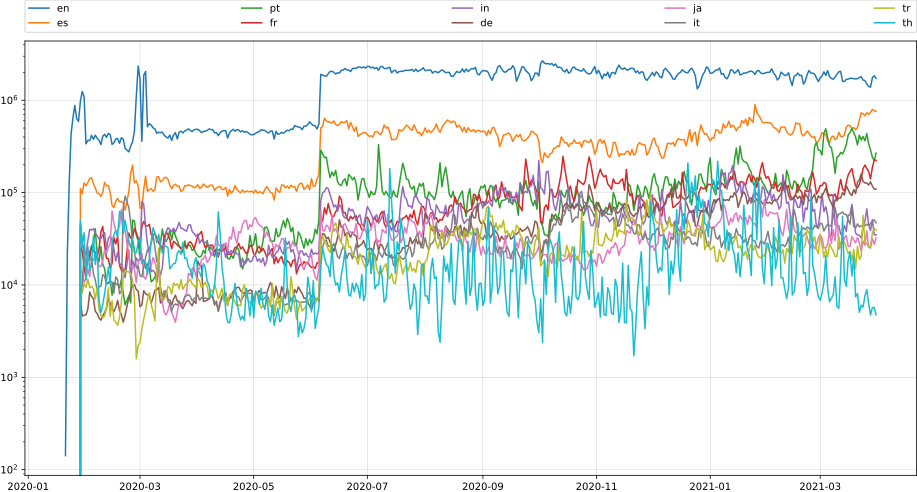
\includegraphics[scale=.4]{tweets_per_language_over_time.svg}
    	\caption{Number of tweets in logarithmic scale over time for the top 10 languages}
    	\label{fig:tweets-language-over-time}
\end{figure}

\section{How to retrieve the data}
\label{sec:retrieve-data}

To comply with Twitter's terms of service,\footnote{\url{https://developer.twitter.com/en/developer-terms/agreement-and-policy}} tweets cannot be released publicly: the repository is in fact a collection of tweet-IDs.

The original tweets can be retrieved, or \textit{hydrated}, using the Python library Twarc with a Twitter Developer Account. In fact, to be able to use the Twitter API, it is mandatory to apply for a Twitter Developer account.\footnote{\url{https://developer.twitter.com/en/apply-for-access}} When the application has been accepted, the developer will be entitled to access the API using tokens. 

Given the id of a tweet, Twarc uses the tokens of the associated developer account to contact the API, and returns the corresponding information as a json object. However, Twarc also tries to maximize the number of possible IDs per request and, at the same time, makes sure to be compliant with the API usage limits.

In the case of this dataset, the data came along with a script to hydrate the tweets automatically.

\section{Tweets}
\label{sec:tweets}
The structure of the Json object for the associated tweet depends on the version of the API used: for this project, we have used Standard v1.1 to hydrate the tweets.\footnote{\url{https://developer.twitter.com/en/docs/twitter-api/v1/data-dictionary/object-model/tweet}}

In general, a tweet is characterized by a number of different fields. For the scope of the project, we decided to keep only the most relevant fields, such as:

\begin{itemize}
	\item \texttt{id}, the integer representation of the unique identifier for this tweet
	\item \texttt{created\_at}, UTC time when this tweet was created
	\item \texttt{full\_text}, the actual UTF-8 text of the status update (not truncated)
	\item \texttt{user}, the user who posted this tweet
	\item \texttt{retweeted\_status}, the presence of this attribute distinguishes retweets from typical tweets
	\item \texttt{favorite\_count}, indicates approximately how many times this tweet has been liked by Twitter users
	\item \texttt{retweet\_count}, number of times this tweet has been retweeted
	\item \texttt{lang}, indicates a BCP 47 language identifier corresponding to the machine-detected language of the tweet text, or und if no language could be detected
\end{itemize}

Further information about the user that posted the tweet are available in the \texttt{user} field, such as:

\begin{itemize}
	\item \texttt{id}, the integer representation of the unique identifier for this user
	\item \texttt{name}, the name of the user, as they have defined it
	\item \texttt{screen\_name}, the screen name, handle, or alias that this user identifies themselves with
	\item \texttt{location}, the user-defined location for this account's profile. Not necessarily a location, nor machine-parseable
	\item \texttt{description}, the user-defined UTF-8 string describing their account
	\item \texttt{default\_profile\_image}, when true, indicates that the user has not uploaded their own profile image and a default image is used instead
	\item \texttt{profile\_image\_url\_https}, a HTTPS-based URL pointing to the user's profile image
	\item \texttt{followers\_count}, the number of followers this account currently has
	\item \texttt{statuses\_count}, the number of tweets (including retweets) issued by the user
\end{itemize}

Given that, each Json object associated with a tweet can be represented as follows:

\begin{lstlisting}[language=Json, caption={Final Json object for a tweet}, captionpos=b, label={lst:tweet_Json}]
{
  "id": 1307025659294674945,
  "full_text": "Here's an article that highlights the updates...",
  "lang": "en",
  "created_at": "Fri Sep 18 18:36:15 +0000 2020",
  "retweet_count": 11,
  "favorite_count": 70,
  "user": {
    "id": 2244994945,
    "id_str": "2244994945",
    "screen_name": "TwitterDev",
    "name": "Twitter Dev",
    "description": "The voice of the #TwitterDev team and your official...",
    "location": "127.0.0.1",
    "followers_count": 513958,
    "statuses_count": 3635,
    "default_profile_image": false,
    "profile_image_url_https": "https:\/\/pbs.twimg.com\/profile_images\/1283786620521652229\/lEODkLTh_normal.jpg"
  }
}
\end{lstlisting}




      \graphicspath{{chapters/chapter3/img/}}

\chapter{Methods}
\label{cha:methods}

This chapter aims to describe all the different methodologies used to analyze the data collected during the previous phase and explained in \autoref{cha:data}. 

The scope of the project is to understand and measure the emotions of the users through sentiment analysis. In particular, we would like to identify, given a certain set of tweets scattered across our considered period of time, when the users conveyed more feelings and which was the emotion expressed the most (e.g. from the Italian tweets it is possible to notice a peak of anger on 21st of February 2020).

Given the heterogeneity of the tweets, we would also like to conduct a more in-dept analysis, by considering the users, over the whole time frame, based on their gender and also on their location.

\section{Lexicons}
\label{lexicons}

Until now we have discussed that we would like to identify and quantify the emotions expressed in the tweets, but we still lack a way to achieve this result. During the project I have used \textit{Lexicons} for this particular task.

The idea behind lexicons is quite simple: we take a particular word in our dictionary, and we assign zero or more emotions or sentiments to it.
\begin{figure}[H]
	\begin{tikzpicture}
		\filldraw (-2,3) node[RectObject, inner xsep=1cm, dashed](pandemic){pandemic};
		\draw (-2,5) node[RectObject, inner xsep=1cm, draw=gray](hospital){hospital};
		\filldraw (8,1) node[RectObject, inner xsep=1cm, line width=0.3mm](negative){negative};
	\filldraw (8,3) node[RectObject, inner xsep=1cm, draw=purple, line width=0.3mm](fear){fear};
		\filldraw (8,5) node[RectObject, inner xsep=1cm, draw=blue, line width=0.3mm](sadness){sadness};
		\filldraw (8,7) node[RectObject, inner xsep=1cm, draw=green, line width=0.3mm](trust){trust};
		\draw[arrow, dashed] (pandemic.east)--(negative.west);
		\draw[arrow, dashed] (pandemic.east)--(fear.west);
		\draw[arrow, dashed] (pandemic.east)--(sadness.west);
		\draw[arrow, draw=gray] (hospital.east)--(trust.west);
		\draw[arrow, draw=gray] (hospital.east)--(fear.west);
		\draw[arrow, draw=gray] (hospital.east)--(sadness.west);
	\end{tikzpicture}
	\caption{Word-emotions/sentiments association}
	\label{fig:word-association}
\end{figure}

However, if we look at \autoref{fig:word-association}, we can notice that, while the word pandemic is associated with only negative emotions/sentiments, the word hospital is associated with fear and sadness but, at the same time, with trust. While this is technically correct, because our lexicon does not know in which context the word is used (i.e. it must consider all the possible meanings), it also introduces a bias.

To simplify even more, even a negation can totally change the meaning of a particular quote:

\begin{center}
	I am fine / I am \underline{not} fine
\end{center}

For this reason, results obtained should be checked and contextualized to get a clear understanding of the situation. 

\paragraph{EmoLex}

For the research, I have used the NRC Word-Emotion Association Lexicon (aka EmoLex) for emotion detection~\cite{ncrwebsite}. EmoLex is a list of English words and their associations with eight basic emotions (anger, fear, anticipation, trust, surprise, sadness, joy, and disgust) and two sentiments (negative and positive).

The peculiarity of this lexicon is the fact that, even if it has been designed for the analysis of English words, it has been translated in over one hundred languages using Google Translates. Given that, the number of different languages identified in the dataset is more than 60, this particular dictionary could perfectly fit our problem.

\section{Data organization}
\label{sub:data-org}

Before performing emotion detection on our tweets, we decided to define a new data organization strategy. In particular,

\begin{itemize}
	\item at the top layer, we sorted the tweets into LANGUAGE folders using the \texttt{lang} field of the json object
	\item then, into YEAR-MONTH folders
	\item finally, we grouped the tweets into files with a prefix “coronavirus-tweet-id-” followed by YEAR-MONTH-DAY
\end{itemize}

The idea behind this partition, aside from considering tweets of the same language, was to get rid of the per hour aggregation: for the purpose of the project, this kind of granularity is simply too much. Given that, we have preferred to aggregate in a single file the tweets posted on the same day.

\autoref{fig:tweet-org-1} shows a visual representation of the new data organization: now it is possible to access directly to tweets of the same language posted on a particular date.

\begin{figure}[H]
	\dirtree{%
		.1 / .
		.2 en.
		.3 2020-01.
		.4 coronavirus-tweet-2020-01-21.json.gz .
		.4 coronavirus-tweet-2020-01-22.json.gz .
		.4 \ldots .
		.4 coronavirus-tweet-2020-01-30.json.gz .
		.4 coronavirus-tweet-2020-01-31.json.gz .
		.3 \ldots .
		.3 2021-03 .
		.4 coronavirus-tweet-2021-03-01.json.gz .
		.4 \ldots .
		.4 coronavirus-tweet-2021-03-31.json.gz .
		.2 it .
		.2 \ldots .
	}
	\caption{First tweets organization}
	\label{fig:tweet-org-1}
\end{figure}

However, this first data organization strategy led to very noisy results: this happened because, depending on the language considered, the number of tweets can drastically change. To solve this problem, we thought about grouping together tweets of the same week: in this way, we were able to average the results more, get stabler data for languages with fewer tweets, and obtain a clearer visualization.

\begin{figure}[H]
	\dirtree{%
		.1 / .
		.2 en.
		.3 coronavirus-tweet-2020-01-20.json.gz .
		.3 coronavirus-tweet-2020-01-27.json.gz .
		.3 \ldots .
		.3 coronavirus-tweet-2021-03-22.json.gz .
		.3 coronavirus-tweet-2021-03-29.json.gz .
		.2 it .
		.2 \ldots .
	}
	\caption{Weekly tweets organization}
	\label{fig:tweet-org-2}
\end{figure}

In this case, the syntax of the files showed in \autoref{fig:tweet-org-2} has a slightly different meaning. In particular, tweets are grouped into files with a prefix “coronavirus-tweet-id-” followed by YEAR-MONTH-FIRST\_WEEK\_DAY.

\section{Valid data}
\label{sec:valid-data}

We have seen in \autoref{sec:period} that the number of retweets in our dataset is much greater than the number of tweets. This could be a problem because if we perform emotion detection with this data, we will end up with a lot of bias. 

Let us suppose to have a particularly positive tweet, for example:

\begin{figure}[H]
	\centering
    	
\includegraphics[scale=.29]{john_doe_tweet.png}
    	\caption{An example of a particularly positive tweet.}
    	\label{fig:tweet-example}
\end{figure}

If John Doe is the only happy person on the 14th of June 2021, then the emotional impact produced from this tweet will not be so significant. Maybe, during that day a lot of people complained on the social network that a streaming platform was not working properly. In this particular case, we will probably find a peak of anger.

However, if John Doe is a celebrity, then the tweet will be surely retweeted thousands of times, and the emotional impact will be much grater. In practice, this means that the previous anger, associated to the malfunctioning of the streaming platform, could pass unnoticed.

To clarify, the fact that a person could retweet a post of a user is not a bad thing: maybe they liked what the original author had written. However, in the case of emotion detection, every words count: if a person agrees with someone's opinion, they will not necessarily use the same exact set of word. In practice, they could still agree with the author of the tweet, but at the same time not convey the same emotion.

For the reasons explained above, we decided to avoid this bias by removing from our dataset all the retweets. As explained in \autoref{sec:tweets},this particular operation can be performed by checking the presence of the \texttt{retweet\_status} field. 


    \endgroup
    % bibliografia in formato bibtex
    %
    % aggiunta del capitolo nell'indice
    \addcontentsline{toc}{chapter}{Bibliography}
    % stile con ordinamento alfabetico in funzione degli autori
    \bibliographystyle{plain}
    \bibliography{biblio}
%%%%%%%%%%%%%%%%%%%%%%%%%%%%%%%%%%%%%%%%%%%%%%%%%%%%%%%%%%%%%%%%%%%%%%%%%%
%%%%%%%%%%%%%%%%%%%%%%%%%%%%%%%%%%%%%%%%%%%%%%%%%%%%%%%%%%%%%%%%%%%%%%%%%%
%% Nota
%%%%%%%%%%%%%%%%%%%%%%%%%%%%%%%%%%%%%%%%%%%%%%%%%%%%%%%%%%%%%%%%%%%%%%%%%%
%% Nella bibliografia devono essere riportati tutte le fonti consultate 
%% per lo svolgimento della tesi. La bibliografia deve essere redatta 
%% in ordine alfabetico sul cognome del primo autore. 
%% 
%% La forma della citazione bibliografica va inserita secondo la fonte utilizzata:
%% 
%% LIBRI
%% Cognome e iniziale del nome autore/autori, la data di edizione, titolo, casa editrice, eventuale numero dell’edizione. 
%% 
%% ARTICOLI DI RIVISTA
%% Cognome e iniziale del nome autore/autori, titolo articolo, titolo rivista, volume, numero, numero di pagine.
%% 
%% ARTICOLI DI CONFERENZA
%% Cognome e iniziale del nome autore/autori (anno), titolo articolo, titolo conferenza, luogo della conferenza (città e paese), date della conferenza, numero di pagine. 
%% 
%% SITOGRAFIA
%% La sitografia contiene un elenco di indirizzi Web consultati e disposti in ordine alfabetico. 
%% E’ necessario:
%%   Copiare la URL (l’indirizzo web) specifica della pagina consultata
%%   Se disponibile, indicare il cognome e nome dell’autore, il titolo ed eventuale sottotitolo del testo
%%   Se disponibile, inserire la data di ultima consultazione della risorsa (gg/mm/aaaa).    
%%%%%%%%%%%%%%%%%%%%%%%%%%%%%%%%%%%%%%%%%%%%%%%%%%%%%%%%%%%%%%%%%%%%%%%%%%
%%%%%%%%%%%%%%%%%%%%%%%%%%%%%%%%%%%%%%%%%%%%%%%%%%%%%%%%%%%%%%%%%%%%%%%%%%
    

    \titleformat{\chapter}
        {\normalfont\Huge\bfseries}{Attachment \thechapter}{1em}{}
    % sezione Allegati - opzionale
    \appendix
    %\chapter{Titolo primo allegato}

Lorem ipsum dolor sit amet, consectetur adipiscing elit. Donec sed nunc orci. Aliquam nec nisl vitae sapien pulvinar dictum quis non urna. Suspendisse at dui a erat aliquam vestibulum. Quisque ultrices pellentesque pellentesque. Pellentesque egestas quam sed blandit tempus. Sed congue nec risus posuere euismod. Maecenas ut lacus id mauris sagittis egestas a eu dui. Class aptent taciti sociosqu ad litora torquent per conubia nostra, per inceptos himenaeos. Pellentesque at ultrices tellus. Ut eu purus eget sem iaculis ultricies sed non lorem. Curabitur gravida dui eget ex vestibulum venenatis. Phasellus gravida tellus velit, non eleifend justo lobortis eget. 

\section{Titolo}
Lorem ipsum dolor sit amet, consectetur adipiscing elit. Donec sed nunc orci. Aliquam nec nisl vitae sapien pulvinar dictum quis non urna. Suspendisse at dui a erat aliquam vestibulum. Quisque ultrices pellentesque pellentesque. Pellentesque egestas quam sed blandit tempus. Sed congue nec risus posuere euismod. Maecenas ut lacus id mauris sagittis egestas a eu dui. Class aptent taciti sociosqu ad litora torquent per conubia nostra, per inceptos himenaeos. Pellentesque at ultrices tellus. Ut eu purus eget sem iaculis ultricies sed non lorem. Curabitur gravida dui eget ex vestibulum venenatis. Phasellus gravida tellus velit, non eleifend justo lobortis eget. 

\subsection{Sottotitolo}
Lorem ipsum dolor sit amet, consectetur adipiscing elit. Donec sed nunc orci. Aliquam nec nisl vitae sapien pulvinar dictum quis non urna. Suspendisse at dui a erat aliquam vestibulum. Quisque ultrices pellentesque pellentesque. Pellentesque egestas quam sed blandit tempus. Sed congue nec risus posuere euismod. Maecenas ut lacus id mauris sagittis egestas a eu dui. Class aptent taciti sociosqu ad litora torquent per conubia nostra, per inceptos himenaeos. Pellentesque at ultrices tellus. Ut eu purus eget sem iaculis ultricies sed non lorem. Curabitur gravida dui eget ex vestibulum venenatis. Phasellus gravida tellus velit, non eleifend justo lobortis eget. 


\chapter{Titolo secondo allegato}

Lorem ipsum dolor sit amet, consectetur adipiscing elit. Donec sed nunc orci. Aliquam nec nisl vitae sapien pulvinar dictum quis non urna. Suspendisse at dui a erat aliquam vestibulum. Quisque ultrices pellentesque pellentesque. Pellentesque egestas quam sed blandit tempus. Sed congue nec risus posuere euismod. Maecenas ut lacus id mauris sagittis egestas a eu dui. Class aptent taciti sociosqu ad litora torquent per conubia nostra, per inceptos himenaeos. Pellentesque at ultrices tellus. Ut eu purus eget sem iaculis ultricies sed non lorem. Curabitur gravida dui eget ex vestibulum venenatis. Phasellus gravida tellus velit, non eleifend justo lobortis eget. 

\section{Titolo}
Lorem ipsum dolor sit amet, consectetur adipiscing elit. Donec sed nunc orci. Aliquam nec nisl vitae sapien pulvinar dictum quis non urna. Suspendisse at dui a erat aliquam vestibulum. Quisque ultrices pellentesque pellentesque. Pellentesque egestas quam sed blandit tempus. Sed congue nec risus posuere euismod. Maecenas ut lacus id mauris sagittis egestas a eu dui. Class aptent taciti sociosqu ad litora torquent per conubia nostra, per inceptos himenaeos. Pellentesque at ultrices tellus. Ut eu purus eget sem iaculis ultricies sed non lorem. Curabitur gravida dui eget ex vestibulum venenatis. Phasellus gravida tellus velit, non eleifend justo lobortis eget. 

\subsection{Sottotitolo}
Lorem ipsum dolor sit amet, consectetur adipiscing elit. Donec sed nunc orci. Aliquam nec nisl vitae sapien pulvinar dictum quis non urna. Suspendisse at dui a erat aliquam vestibulum. Quisque ultrices pellentesque pellentesque. Pellentesque egestas quam sed blandit tempus. Sed congue nec risus posuere euismod. Maecenas ut lacus id mauris sagittis egestas a eu dui. Class aptent taciti sociosqu ad litora torquent per conubia nostra, per inceptos himenaeos. Pellentesque at ultrices tellus. Ut eu purus eget sem iaculis ultricies sed non lorem. Curabitur gravida dui eget ex vestibulum venenatis. Phasellus gravida tellus velit, non eleifend justo lobortis eget. 




\end{document}
